\section{Results}
\label{subsec:cupid-results}
A number of examples of the application of \ac{CUPID} are now provided.
For details relating to generation of the datasets, see Sections
\ref{sec:simulated-datasets} and \ref{subsec:cupid-experimental}. Useful
metrics, such a run times and the number of oscillators present at different
stages of the routine are provided in Table \ref{tab:cupid-metrics}.

\subsection{``Four Multiplets''}
\label{subsec:four-mp}
\begin{figure}
    \centering
    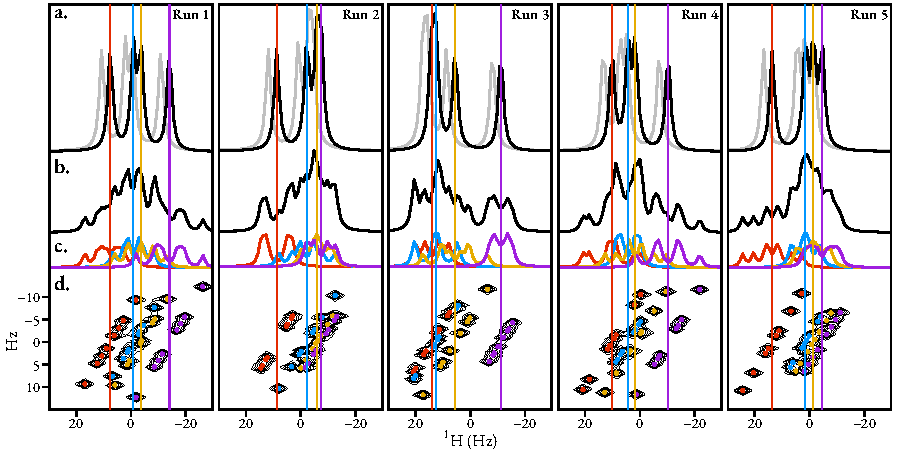
\includegraphics{four_multiplets/four_multiplets}
    \caption[
        The result of applying \acs{CUPID} to 5 instances of simulated
        \acs{2DJ} datasets with 4 heavily overlapping multiplet structures.
    ]{
        The result of applying \ac{CUPID} to 5 instances of simulated \ac{2DJ}
        datasets with 4 heavily overlapping multiplet structures.
        \textbf{a.} Black: pure shift spectrum generated by \ac{CUPID} (via the
        \ang{-45} signal).
        Grey: \ac{1D} spectrum simulated with Spinach, using the same spin
        system as was used to produce the \ac{2DJ} dataset, but with all scalar
        couplings set to \qty{0}{\hertz}. This has been offset slightly for
        clarity.
        \textbf{b.} \ac{1D} spectrum of the dataset, produced using the first
        direct-dimension \ac{FID} in the \ac{2DJ} dataset.
        \textbf{c.} Multiplet structures predicted, using a threshold $\epsilon
        = \nicefrac{\fswtwo}{\Ntwo} \approx \qty{0.98}{\hertz}$.
        \textbf{d.} Contour plot of the magnitude-mode \ac{2DJ} spectrum.
        Coloured points denote the frequencies of oscillators in the
        estimation result. Coloured vertical lines denote the predicted central
        frequencies of each multiplet structure.
    }
    \label{fig:four-multiplets}
\end{figure}
A series of five simulated \proton\ \ac{2DJ} datasets
were generated using \textsc{Spinach} such that within a
known region of the spectrum four ddd multiplet structures with significant
overlap were present. The simulations were conducted with a field strength of
\qty{500}{\mega\hertz}, and the region of interest was
\SIrange{-30}{30}{\hertz}, equivalent to
\SIrange{-0.06}{0.06}{\partspermillion}. The spin systems used to produce the
dataset were generated in a similar fashion to the inversion recovery example
in Section \ref{subsec:seq-results}, with four ``estimated'' and three
``coupling'' spins:
\begin{itemize}
    \item The estimated spins were assigned chemical shifts randomly
        sampled from $\mathcal{U}(\qty{-0.03}{\partspermillion},
        \qty{0.03}{\partspermillion})$.
    \item The coupling spins were assigned chemical shifts $\gg
        \qty{0.06}{\partspermillion}$, and were coupled to each of the
        estimated spins, with the values of the couplings randomly sampled from
        $\mathcal{U}(\qty{-10}{\hertz}, \qty{10}{\hertz})$.
\end{itemize}
\ac{AWGN} was added to the \ac{FID}, with a target \ac{SNR} of \qty{30}{\deci\bel}.
A filtered sub-\ac{FID} containing only the signals from the estimated spins
was then generated using the described filtering procedure, with the left and
right bounds of the region of interest being \qty{0.06}{\partspermillion} and
\qty{-0.06}{\partspermillion}, respectively.
The resulting sub-\ac{FID} was expected to comprise 32 ($4 \times
2^3$) signals. As can be seen in Figure
\ref{fig:four-multiplets}.b, the first direct-dimension \acp{FID} of these
datasets are too crowded for reasonable estimates of model order to be made
using the \ac{MDL}, so a value was manually provided. For each run, a random
integer from the range $[33, 40]$ was selected as the initial number of
oscillators. Hence, the initial guess from the \ac{MMEMPM} would comprise a
slightly excessive number of oscillators. Each \ac{FID} was subjected to
estimation, yielding the result vector $\bthstar$. Oscillators unlikely to be
related to first-order signals were checked for, using the criteria outlined in
Section \ref{subsec:mp-selection}, with the threshold for multiplet assignment
set to the spectral resolution in the direct dimension: $\epsilon =
\nicefrac{f_{\text{sw}}^{(2)}}{\Ntwo}$. If any of these oscillators were found,
these were removed from the result.

Figure \ref{fig:four-multiplets} illustrates the result achieved for each of
the runs. For each \ac{FID} generated, the method was effective at producing an
estimation result with 32 oscillators, as desired, despite the excessive number
that were present in $\bthzero$. Most of the excessive oscillators were purged
from $\bthzero$ through the \ac{NLP} procedure.
For 2 of the 5 datasets, the result after \ac{NLP} comprised 33
oscillators, with a single oscillator being associated with noise. These were
automatically detected and removed. With simulated examples, it is easy to
confirm that the pure shift spectrum generated using \ac{CUPID} agrees with the
expected pure shift spectrum; it is possible to generate the ``true'' pure shift
spectrum by simulating a pulse-acquire experiment with \textsc{Spinach}, using
a spin system with same chemical shifts, but all scalar couplings set to
\qty{0}{\hertz}.
As seen in Figure \ref{fig:four-multiplets}.a. the spectra produced
using \ac{CUPID} agree well with these.

% \subsection{Sucrose simulated}
% \label{subsec:sucrose-cupid}
% \note{Maybe not so impressive? Perhaps try strychnine?}
% \begin{figure}
%     \centering
%     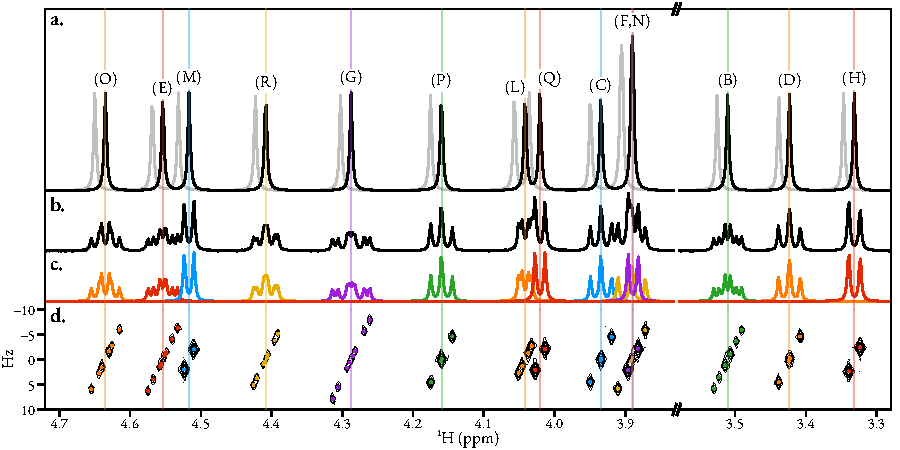
\includegraphics{sucrose_cupid/sucrose_cupid.pdf}
%     \caption[
%         Application of \acs{CUPID} on a simulated sucrose \acs{2DJ} dataset.
%     ]
%     {
%         Application of \ac{CUPID} on a simulated sucrose \ac{2DJ} dataset.
%         \textbf{a.} Black: the spectrum generated from \ac{FT} of the \ang{-45}
%         signal. Grey: the spectrum of a simulated dataset with the same
%         chemical shifts, with all scalar couplings set to \qty{0}{\hertz}.
%         \textbf{b.} Conventional \ac{1D} spectrum.
%         \textbf{c.} Multiplet structures assigned ($\epsilon \approx
%         \qty{0.27}{\hertz}$).
%         \textbf{d.} Contour plot of the absolute value mode \ac{2DJ} spectrum,
%         with the locations of assigned oscillators given as coloured points.
%     }
%     \label{fig:sucrose-cupid}
% \end{figure}
% As a second example of applying \ac{CUPID} on simulated data, the chemical
% shifts and isotropic scalar couplings associated with a
% Gaussian\cite{Gaussian03} \ac{DFT} calculation of sucrose in a vacuum
% \footnote{
% It is well known that isotropic chemical shift calculations using \ac{DFT} are
% typically very inaccurate. The resulting spectrum is not typical of sucrose in
% the liquid state, though this doesn't really matter for assessing the
% performance of \ac{CUPID}.
% }
% were used to construct a 2DJ dataset. \ac{AWGN} was added with a target
% \ac{SNR} of \qty{20}{\deci\bel}. The CUPID procedure was applied to filtered
% sub-FIDs such that the signals arising from all 22 spins were considered, though
% only the regions of the dataset with the most interesting multiplet structures
% are presented in Figure \ref{fig:sucrose-cupid}.

% The estimation technique successfully assigned multiplet structures for all 22
% multiplets in the dataset, including structures derived from two spins (F \& N)
% with a \qty{0.6}{\hertz} difference in resonance frequency, approaching the
% spectral resolution in the direct dimension (\qty{0.537}{\hertz}). The
% pure-shift spectrum generated via the \ang{-45} signal again showed close
% agreement with a 1D spectrum simulated using the same chemical shifts, with
% scalar couplings set to \qty{0}{\hertz}. There are particular multiplets where
% the number of oscillators fit using the estimation routine was less than the
% true number. Examples of this phenomenon are exhibited in the estimates of the
% multiplets for spins B \& O, which are both ddd structures. The scalar
% couplings involved meant that certain oscillators were
% of such similar frequencies that they were separated by significantly less than
% the spectral resolution, and thus resolving these was unrealistic. For
% example, there are two pairs of peaks in the spin-B multiplet which lie only
% \qty{0.085}{\hertz} apart. Under-fitting in this case had a negligible impact
% on the final pure shift spectrum. However there are circumstances which will be
% seen in the experimental examples below where more blatant cases of under-fitting
% lead to the generation of peaks in the pure shift spectrum which are noticeably
% broadened.

\subsection{Strychnine simulated}
\label{subsec:strychnine-cupid}
\begin{figure}
    \centering
    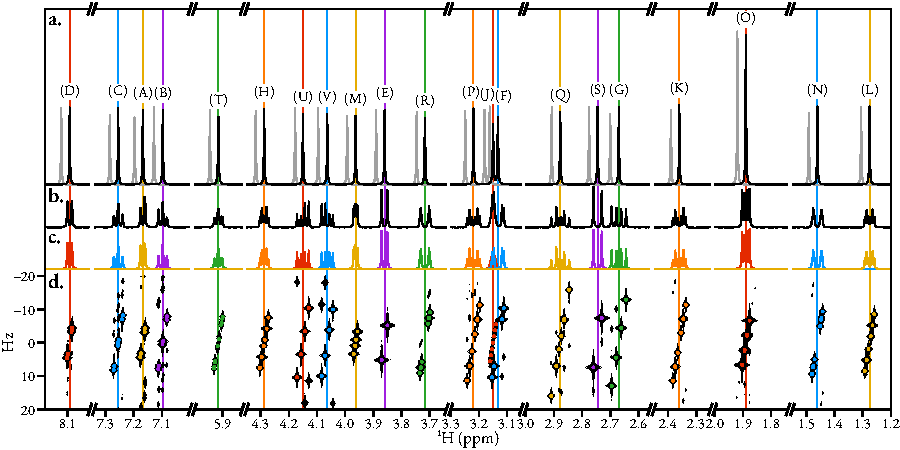
\includegraphics{strychnine_cupid/strychnine_cupid.pdf}
    \caption[
        Application of \acs{CUPID} on a simulated strychnine \acs{2DJ} dataset.
    ]
    {
        Application of \ac{CUPID} on a simulated strychnine \ac{2DJ} dataset.
        \textbf{a.} Black: the spectrum generated from \ac{FT} of the \ang{-45}
        signal. Grey: the spectrum of a simulated dataset with the same
        chemical shifts, with all scalar couplings set to \qty{0}{\hertz}.
        \textbf{b.} Conventional \ac{1D} spectrum.
        \textbf{c.} Multiplet structures assigned ($\epsilon =
        \nicefrac{\fswone}{\None} \approx \qty{0.39}{\hertz}$).
        \textbf{d.} Contour plot of the absolute value mode \ac{2DJ} spectrum,
        with the locations of assigned oscillators given as coloured points.
    }
    \label{fig:strychnine-cupid}
\end{figure}
As a second example of applying \ac{CUPID} on simulated data, the chemical
shifts and isotropic scalar couplings associated with strychnine
were used to construct a 2DJ dataset at \qty{500}{\mega\hertz}. \ac{AWGN} was
include with a target
\ac{SNR} of \qty{20}{\deci\bel}. The CUPID procedure was applied to filtered
sub-FIDs such that the signals arising from all spins were considered, with the
result presented in Figure \ref{fig:strychnine-cupid}. There are numerous
regions in the dataset where strong coupling artefacts reside, and as such this
dataset provides a good gauge on the effectiveness on \ac{CUPID} when these are
present.

The \ac{MDL} was applied to the first direct-dimension \ac{FID} in order to
predict model order. In most circumstances, the model order used resulted
in estimation results in which the first-order signals have been well
quantified, while those corresponding to strong coupling artefacts are almost
entirely neglected.
The resulting pure shift spectrum is therefore largely devoid
of small intensity nuisance peaks which would exist if the artefacts were
included in the estimation result. There are a few occasions where strong
coupling artefacts are included in the estimation result; the relevant
oscillators are denoted in grey in Figure \ref{fig:strychnine-cupid}. The
absence of strong coupling artefacts in the estimation result also leads to
generated multiplet structures which do not exhibit the typical ``roofing''
phenomenon associated with strongly coupled spins (\textit{cf.} panels b and c of
Figure \ref{fig:strychnine-cupid}). The clearest examples of this are
associated with spins (U) \& (V), as well as (A), (B) \& (C). As with the
``four multiplets'' example, good agreement is achieved between the pure shift
spectrum generated via the \ang{-45} signal, and a spectrum generated by
running a \ac{1D} simulation with the same spin system, and scalar couplings
set to \qty{0}{\hertz}.

\subsection{Quinine}
\begin{figure}
    \centering
    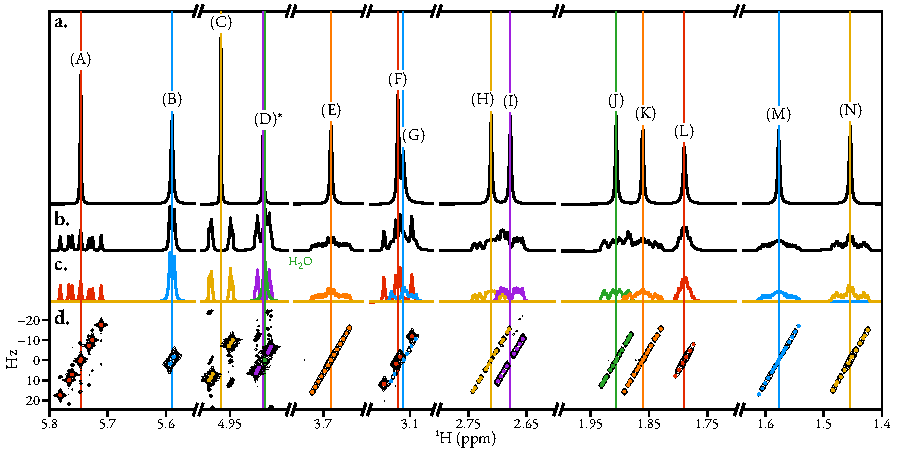
\includegraphics{quinine_cupid/quinine_cupid.pdf}
    \caption[
        Application of \acs{CUPID} on the non-aromatic regions of a quinine
        \acs{2DJ} dataset.
    ]{
        Application of \ac{CUPID} on the non-aromatic regions of a quinine
        \ac{2DJ} dataset.
        \textbf{a.} Spectrum produced using the \ang{45} shear and summation
        methodology. The peaks denoted by and asterisk arise from string
        coupling artefacts.
        \textbf{b.} The spectrum generated from \ac{FT} of the \ang{-45}
        signal, with the signal arising from H\textsubscript{2}O (grey, close
        to \qty{4.9}{\partspermillion} neglected).
        \textbf{c.} Spectrum of the first direct-dimension signal in the
        \ac{2DJ} \ac{FID}.
        \textbf{d.} Multiplet structures assigned ($\epsilon =
        \nicefrac{\fswtwo}{\Ntwo} \approx \qty{0.92}{\hertz}$).
        \textbf{e.} Contour plot of the absolute value mode \ac{2DJ} spectrum,
        with the locations of assigned oscillators given as coloured points.
    }
    \label{fig:quinine-cupid}
\end{figure}

Figure \ref{fig:quinine-cupid} illustrates the result of applying \ac{CUPID} on
a dataset generated from a sample comprising quinine (Figure
\ref{fig:structures}.a) in CD\textsubscript{3}OD,
with all signals arising from non-aromatic protons considered. The method
successfully generated a pure shift spectrum with distinct peaks for each
\textsuperscript{1}H environment.
Another example of strong coupling artefacts not being quantified can be seen
around the \qty{4.9}{\partspermillion} region, featuring signals from spins (C)
\& (D). As well as this, the multiplet grouping procedure is able to separate
the signals corresponding to spin (D) (purple) and residual water in the sample
(grey).
The presence of water is a hindrance since it heavily overlaps with (D)'s
multiplet structure.
To obtain a clean singlet for spin (D) in the pure shift spectrum, the
oscillator corresponding to the water signal was simply neglected from
the parameter set used to generate the \ang{-45} signal. This concept of
neglecting nuisance signals through post-processing has similarities with
\ac{SVD}-based approaches for solvent suppression\cite{Zhu1997}\footnote{
    Solvent suppression approaches of this manner tend to operate by assuming
    that the most significant component(s) in the data are derived from the
    solvent. The relevant component(s) are subtracted from the dataset to
    remove their influence. The removal of the water signal is slightly
    different here, in that it was removed manually (rather than automatically)
    by inspecting the result of \ac{CUPID}.
    A knowledgeable user would be able to locate the water signal, determine
    that it is undesirable, and neglect it.
}.

This example provides a few examples where a noticeable under-fitting of
multiplet structures has occurred.
The most notable case comes from the spin (G) multiplet, where close proximity
with spin (F)'s multiplet has likely compounded the task of accurately
estimating the associated signals. With fewer oscillators than the true number
of signals at its disposal, the \ac{NLP} routine will compensate
by giving said oscillators large amplitudes and damping factors, so that they
can reasonably fit multiple similar-frequency signals. This phenomenon
culminates in the pure shift peak possessing an augmented linewidth.
This behaviour is also exhibited to a lesser extent by the multiplet for spin
(B), which comprises two pairs of very close signals in a dd structure. A
single oscillator is fit to each pair of signals, culminating in a broadened
pure shift peak. While linewdiths are affected by under-fitting hard-to-resolve
multiplets, the integrals of the pure shift peaks are not typically perturbed
significantly.

For comparison, panel a of Figure \ref{fig:quinine-cupid} presents a pure-shift
spectrum produced via application of a \ang{45} shear, followed by summation
along the indirect dimension. Due to the application of sine-bell apodisation,
the relative amplitudes of the pure-shift peaks are drastically different.
In particular, the alkenyl signals from spins (A), (C) \& (D), are less
perturbed by the apodisation relative to the aliphatic signals due to longer
$T_2$ times\footnote{
    Spins with longer $T_2$s produce signals which decay less rapidly.
    Sine-bell apodisation diminishes the amplitudes of the initial points in
    the \ac{FID}. Therefore, if the signal decays less rapidly, the relative
    extent by which the \emph{power} of the signal is diminished is less
    compared with a signal derived from a spin with a small $T_2$.
}. As well as this, signals arising from strong coupling between (C) and
(D) are visible (these are denoted with an asterisk).

\subsection{Camphor}
\begin{figure}%
    \centering%
    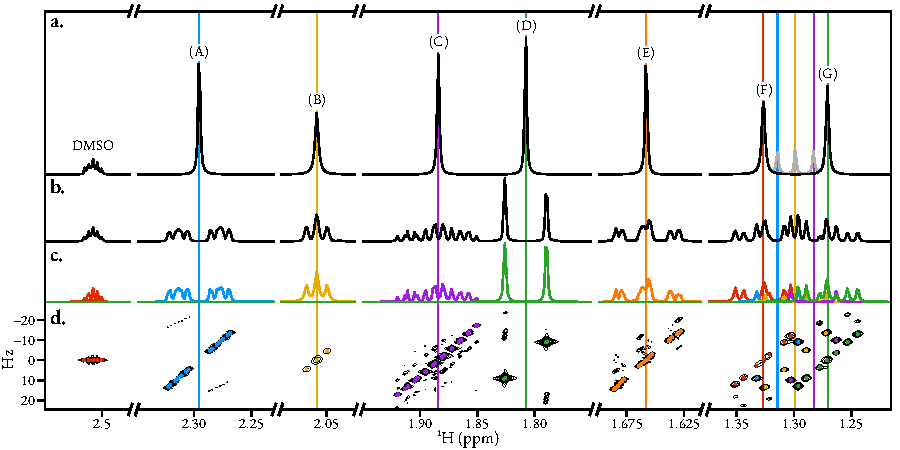
\includegraphics{camphor_cupid/camphor_cupid.pdf}%
    \caption[
        Application of \acs{CUPID} on a camphor dataset.
    ]{
        Application of \acs{CUPID} on camphor \ac{2DJ} dataset.
        \textbf{a.} Black: the spectrum generated from \ac{FT} of the \ang{-45}
        signal. Oscillators associated with strong coupling artefacts between
        spins (F) and (G) were neglected. Grey: spectrum generated without
        neglecting oscillators associated with strong coupling artefacts.
        \textbf{b.} \acs{1D} spectrum produced from the first direct-dimension
        \ac{FID} in the dataset. Note that, unlike a conventional pulse-acquire
        spectrum, strong coupling artefacts are present.
        \textbf{c.} Multiplet structures assigned ($\epsilon =
        \nicefrac{2 \fswtwo}{\Ntwo} \approx \qty{1.23}{\hertz}$).
        \textbf{d.} Contour plot of the absolute value mode \acs{2DJ} spectrum,
        with the locations of assigned oscillators given as coloured points.
    }
    \label{fig:camphor-cupid}%
\end{figure}%
\note{Are the signals that I neglect in the final pure shift spectrum definitely due to strong coupling?}
The application of \ac{CUPID} to the non-methyl regions of a \ac{2DJ}
dataset of camphor (Figure \ref{fig:structures}.c) in \acs{DMSOd6} is presented
in Figure \ref{fig:camphor-cupid}. As in the quinine case, there are instances
of underfitting poorly resolved multiplets, resulting in broadened pure shift peaks.
The peak associated with spin (B) is the most drastic case here, where 4
vicinal couplings to protons with dihedral angles of \ang{60} are present,
along with potentially more contributions from long range couplings.
This example highlights the ability of \ac{CUPID} to remove another class of nuisance peak: \emph{strong coupling artefacts}\footnote{
    As stressed in \cite{Thrippleton2005}, these are not strictly artefacts,
    but rather genuine signals, which are expected to be present in the
    \ac{2DJ} dataset. Despite this, the term is widespread in the literature.
},
which arise due to mixing effects induced by the \ang{180} pulse in the
\ac{2DJ} sequence\cite{Thrippleton2005,Wider1983}.
The effects of strong coupling lead to the presence of extra unexpected signals
which do not agree with the chemical shift of any spin associated with camphor.
An example of this is found between \SIrange{1.35}{1.25}{\partspermillion} in
the \ac{2DJ} spectrum, where artefacts associated with spins (F) and (G) are
located.
The estimation routine was able to determine parameters for
the more intense signals which comprise the strong coupling artefacts (these
are coloured blue, yellow, and purple, while oscillators associated with the
true multiplet structures for (F) and (G) are coloured red and green, respectively).
Inclusion of all oscillators extracted by the estimation routine generates the
spectrum in panel a, with the low-intensity grey peaks associated with the strong
coupling effects included. However, in much the same way as the water signal in
the quinine example could be neglected, it is trivial to construct the \ang{-45}
signal with the oscillators associated with strong coupling artefacts left out,
which produces the black spectrum.

\subsection{Dexamethasone}
\begin{sidewaysfigure}%
    \centering%
    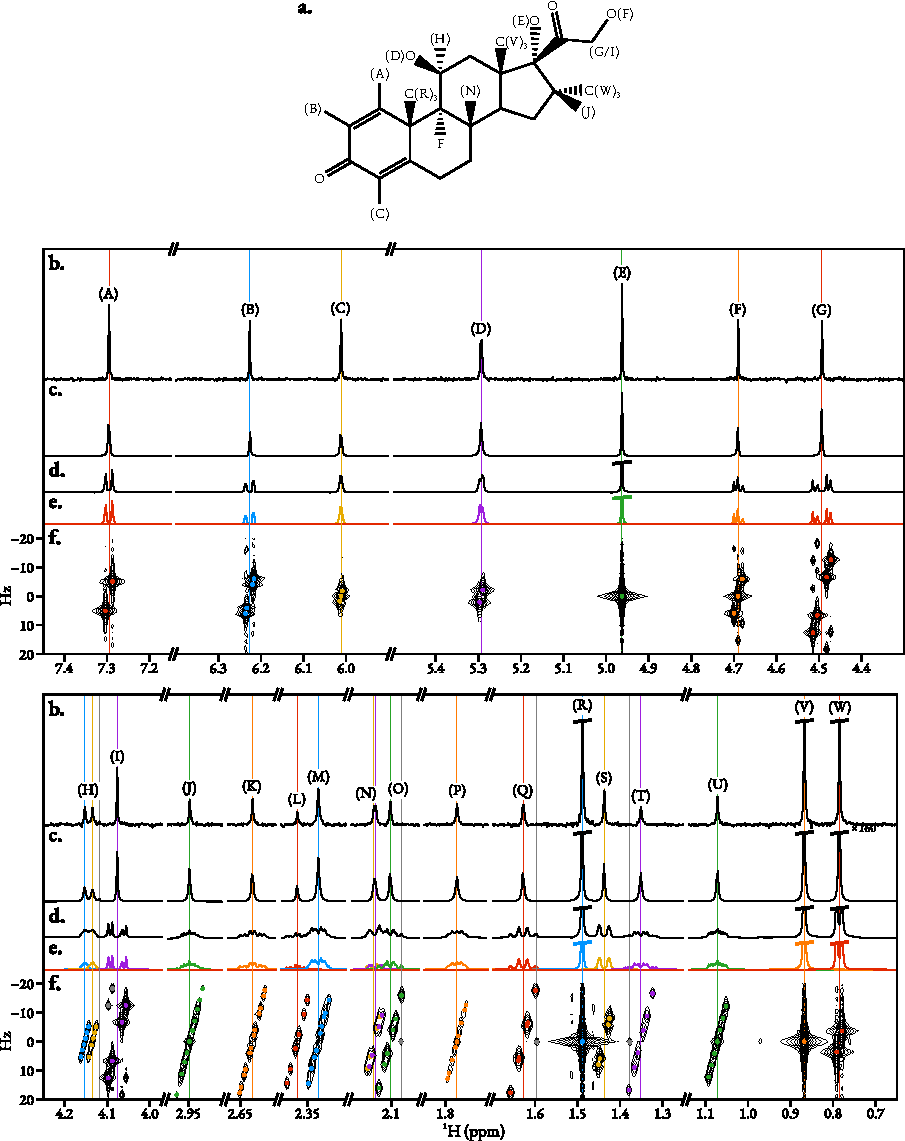
\includegraphics{dexamethasone_cupid/dexamethasone_cupid.pdf}%
    \caption[
        Application of \acs{CUPID} on a dexamethasone dataset.
    ]{
        \note{Fix magnification label.}
        Application of \acs{CUPID} on dexamethasone \ac{2DJ} dataset.
        \textbf{a.} \acs{TSE-PSYCHE} spectrum of the sample.
        \textbf{b.} The spectrum generated from \ac{FT} of the \ang{-45}
        signal.
        \textbf{c.} Conventional \acs{1D} spectrum.
        \textbf{.} Multiplet structures assigned ($\epsilon =
        \nicefrac{\fswtwo}{\Ntwo} \approx \qty{0.92}{\hertz}$).
        \textbf{d.} Contour plot of the absolute value mode \acs{2DJ} spectrum,
        with the locations of assigned oscillators given as coloured points.
    }
    \label{fig:dexamethasone-cupid}%
\end{sidewaysfigure}%

Figure \ref{fig:dexamethasone-cupid} shows the result of applying CUPID on a
dataset acquired from a sample dexamethasone in DMSO-d\textsubscript{6}. A
pure-shift spectrum was also acquired using the
\ac{TSE-PSYCHE} experiment\cite{Foroozandeh2018,Foroozandeh2015} for
comparison.
\ac{CUPID} generated a pure-shift spectrum with overall excellent agreement
with the \ac{TSE-PSYCHE} spectrum. Certain multiplet structures in the spectrum exhibit
splitting in the direct dimension, on account of heteronuclear couplings to
\textsuperscript{19}F. Most notable are those derived from spins (D), (H) \& (O). For the (D) multiplet, the
magnitude of the heterocoupling is very small such that assigning these to
separate oscillators was not achievable.
For the spin (N) multiplet, two separate structures were successfully assigned
(see the orange and green multiplets around \qty{2.1}{\partspermillion}).
The estimation routine was unsuccessful at accurately estimating the structure
associated with spin (H), where a severe under-fitting occurred. An under-fitting
of this structure even occurred when the estimation was re-run using
considerable over-estimation of the model order, with most oscillators in the
initial guess being purged during the \ac{NLP} procedure.
The spin (H) multiplet provides an extreme example line-broadening in the pure
shift spectrum on account of under-fitting. The most downfield peaks in the
CUPID spectrum (corresponding to aromatic and hydroxyl protons) also appear to
be noticeably broadened relative to their PSYCHE equivalents. This is also
probably due to under-fitting of the relevant multiplet structures, though to a
far less noticeable extent than for spin H. \note{Any other reason why this
might be so?}

\subsection{Estradiol}
\begin{figure}
    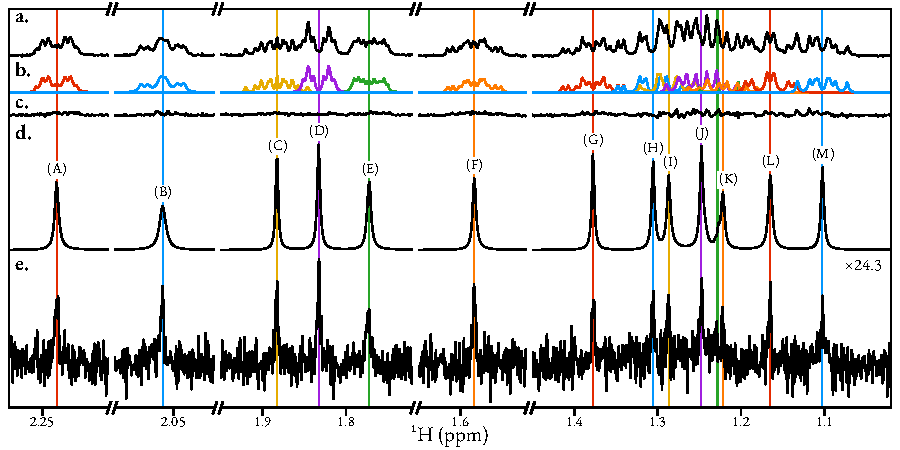
\includegraphics{estradiol_cupid/estradiol_cupid.pdf}%
    \caption[
        Application of \acs{CUPID} on a 17\textbeta-estradiol dataset.
    ]{
        Application of \acs{CUPID} on \ac{2DJ} dataset of 17\textbeta-estradiol
        in \acs{DMSOd6}.
        \textbf{a.} Spectrum of the first direct-dimension \ac{FID} in the
        \ac{2DJ} dataset.
        \textbf{b.} Multiplet structures assigned ($\epsilon =
        \nicefrac{\fswtwo}{\Ntwo} \approx \qty{2}{\hertz}$).
        \textbf{c.} The residual between the spectrum in panel a and the lines
        in panel b.
        \textbf{d.} The pure shift spectrum generated using \ac{CUPID}.
        \textbf{e.} \acs{PSYCHE} spectrum of the sample see Figure
        \ref{fig:psyche} for details on the pulse sequence. The spectrum has
        been scaled such that the maximum is of the same magnitude as the
        corresponding point in the \ac{CUPID} spectrum.
    }
    \label{fig:estradiol-cupid}%
\end{figure}

A final showcase of \ac{CUPID} is provided by Figure \ref{fig:estradiol-cupid}, where a low concentration (\qty{2}{\milli\molar}) sample of 17\textbeta-estradiol (Figure \ref{fig:structures}.
